In this experiment we consider 4 different finite elements. The idea behind this stone 
is to build a code which code(the FEM build and assembly) is common to all. 
The setup is the Donea \& HUerta benchmark (Section~\ref{mms1}), which has been modified so that 
the pressure is zero at the top right corner.

\begin{verbatim}

Q4xQ3                    Q3xQ2                  Q2xQ1                 Q1Q0

20===21===22===23===24  12====13====14====15  06======07=======08  02===============03
|                    |  |      |     |     |  |        |        |  |                 |
|                    |  |      |     |     |  |        |        |  |                 |
20===21===22===23===24  |      |     |     |  |        |        |  |                 |
|                    |  08====09====10====11  |        |        |  |                 |
|                    |  |      |     |     |  |        |        |  |                 |
20===21===22===23===24  |      |     |     |  03======04=======05  |                 |
|                    |  |      |     |     |  |        |        |  |                 |
|                    |  04====05====06====07  |        |        |  |                 |
20===21===22===23===24  |      |     |     |  |        |        |  |                 |
|                    |  |      |     |     |  |        |        |  |                 |
|                    |  |      |     |     |  |        |        |  |                 |
20===21===22===23===24  00====01====02====03  00======01=======02  00===============01 

12====13=====14=====15  06=======07=======08  02===============03  .=================.
|      |      |      |  |        |         |  |                 |  |                 |
|      |      |      |  |        |         |  |                 |  |                 |
|      |      |      |  |        |         |  |                 |  |                 |
08====09=====10=====11  |        |         |  |                 |  |                 |
|      |      |      |  |        |         |  |                 |  |                 |
|      |      |      |  03=======04=======05  |                 |  |       00        |
|      |      |      |  |        |         |  |                 |  |                 |
04====05=====06=====07  |        |         |  |                 |  |                 |
|      |      |      |  |        |         |  |                 |  |                 |
|      |      |      |  |        |         |  |                 |  |                 |
|      |      |      |  |        |         |  |                 |  |                 |
00====01=====02=====03  00=======01=======02  00===============01  .=================.

mV=25, mP=16            mV=16, mP=9           mV=9, mP=4           mV=4, mP=1      

\end{verbatim}

In the code the 'order' parameter can take values 1,2,3 and 4 which 
correspond to the polynomial order of the velocity approximation ($Q_1$, $Q_2$, $Q_3$ and $Q_4$).

When both nelx and nely values have been chosen, the total number of element 
for a regular 2D grid is simply:
\begin{lstlisting}
nel=nelx*nely
\end{lstlisting}

The number of nodes in each direction is then easily computed:
\begin{lstlisting}
nnx=order*nelx+1 
nny=order*nely+1 
\end{lstlisting}
and so is then the total number of velocity nodes:
\begin{lstlisting}
NV=nnx*nny
\end{lstlisting}

The total number of pressure nodes is as follows:
\begin{lstlisting}
if order==1:
   NP=nelx*nely
if order==2:
   NP=(nelx+1)*(nely+1)
if order==3:
   NP=(2*nelx+1)*(2*nely+1)
if order==4:
   NP=(3*nelx+1)*(3*nely+1)
\end{lstlisting}

Each velocity node has 2 dofs (ndofV=2) while pressure nodes have one dof (ndofP=1) so that 
the size of the blocks and the assembled FE matrix are given by:

\begin{lstlisting}
NfemV=NV*ndofV      
NfemP=NP*ndofP    
Nfem=NfemV+NfemP
\end{lstlisting}

For the linear element, 2 quadrature points per dimension are enough (nqperdim=2), 
while 3 are necessary for the quadratic element (nqperdim=3) and 4 are used  
for the cubic element (nqperdim=4), and 5 for the quartic element,
which can be conveniently implemented as follows:
\begin{lstlisting}
nqperdim=order+1
\end{lstlisting}
The quadrature points location and weight is document in Section~\ref{sec:quadrature}.

Because we wish to use a regular grid, the layout of the points for all three elements 
can be implemented easily:

\begin{lstlisting}
counter=0    
for j in range(0,nny):
    for i in range(0,nnx):
        xV[counter]=i*hx/order
        yV[counter]=j*hy/order
        counter+=1
\end{lstlisting}

The position of the pressure nodes follows a similar logic.

When it comes to the connectivity array, I first started by building it 
for each element as follows:

\begin{lstlisting}
if order==1:
   counter=0
   for j in range(0,nely):
       for i in range(0,nelx):
           iconV[0,counter]=(i)*1+0+(j)*1*nnx+nnx*0 
           iconV[1,counter]=(i)*1+1+(j)*1*nnx+nnx*0 
           iconV[2,counter]=(i)*1+0+(j)*1*nnx+nnx*1 
           iconV[3,counter]=(i)*1+1+(j)*1*nnx+nnx*1 
           counter += 1

if order==2:
   counter = 0
   for j in range(0,nely):
       for i in range(0,nelx):
           iconV[0,counter]=(i)*2+0+(j)*2*nnx+nnx*0 
           iconV[1,counter]=(i)*2+1+(j)*2*nnx+nnx*0 
           iconV[2,counter]=(i)*2+2+(j)*2*nnx+nnx*0 
           iconV[3,counter]=(i)*2+0+(j)*2*nnx+nnx*1 
           iconV[4,counter]=(i)*2+1+(j)*2*nnx+nnx*1 
           iconV[5,counter]=(i)*2+2+(j)*2*nnx+nnx*1 
           iconV[6,counter]=(i)*2+0+(j)*2*nnx+nnx*2 
           iconV[7,counter]=(i)*2+1+(j)*2*nnx+nnx*2
           iconV[8,counter]=(i)*2+2+(j)*2*nnx+nnx*2 
           counter += 1

if order==3:
   counter = 0
   for j in range(0,nely):
       for i in range(0,nelx):
           iconV[ 0,counter]=(i)*3+0+(j)*3*nnx+0*nnx 
           iconV[ 1,counter]=(i)*3+1+(j)*3*nnx+0*nnx 
           iconV[ 2,counter]=(i)*3+2+(j)*3*nnx+0*nnx 
           ...
           iconV[13,counter]=(i)*3+1+(j)*3*nnx+3*nnx 
           iconV[14,counter]=(i)*3+2+(j)*3*nnx+3*nnx 
           iconV[15,counter]=(i)*3+3+(j)*3*nnx+3*nnx 
           counter += 1
\end{lstlisting}
Having done so, it becomes quickly apparent that the connectivity array 
can be computed for all elements as follows:
\begin{lstlisting}
counter=0
for j in range(0,nely):
    for i in range(0,nelx):
        counter2=0
        for k in range(0,order+1):
            for l in range(0,order+1):
                iconV[counter2,counter]=i*order+l+j*order*nnx+nnx*k
                counter2+=1
        counter += 1
\end{lstlisting}
The same approach is taken to build the pressure connectivity array, 
although the $Q_1\times P_0$ element requires special attention since
the pressure is elemental and attributed to a single node inside the element. 

For the other elements I started from:

\begin{lstlisting}
if order==2:
   counter=0
   for j in range(0,nely):
       for i in range(0,nelx):
           iconP[0,counter]=(i)*1+0+(j)*1*(nelx+1)+(nelx+1)*0 
           iconP[1,counter]=(i)*1+1+(j)*1*(nelx+1)+(nelx+1)*0 
           iconP[2,counter]=(i)*1+0+(j)*1*(nelx+1)+(nelx+1)*1 
           iconP[3,counter]=(i)*1+1+(j)*1*(nelx+1)+(nelx+1)*1 
           counter += 1

if order==3:
   counter=0
   for j in range(0,nely):
       for i in range(0,nelx):
           iconP[0,counter]=(i)*2+0+(j)*2*(2*nelx+1)+(2*nelx+1)*0 
           iconP[1,counter]=(i)*2+1+(j)*2*(2*nelx+1)+(2*nelx+1)*0 
           iconP[2,counter]=(i)*2+2+(j)*2*(2*nelx+1)+(2*nelx+1)*0 
           iconP[3,counter]=(i)*2+0+(j)*2*(2*nelx+1)+(2*nelx+1)*1 
           iconP[4,counter]=(i)*2+1+(j)*2*(2*nelx+1)+(2*nelx+1)*1 
           iconP[5,counter]=(i)*2+2+(j)*2*(2*nelx+1)+(2*nelx+1)*1 
           iconP[6,counter]=(i)*2+0+(j)*2*(2*nelx+1)+(2*nelx+1)*2 
           iconP[7,counter]=(i)*2+1+(j)*2*(2*nelx+1)+(2*nelx+1)*2 
           iconP[8,counter]=(i)*2+2+(j)*2*(2*nelx+1)+(2*nelx+1)*2 
           counter += 1

if order==4:
   etc ...
\end{lstlisting}
and quickly arrived at the following compact form:
\begin{lstlisting}
if order>1:
   om1=order-1
   counter=0
   for j in range(0,nely):
       for i in range(0,nelx):
           counter2=0
           for k in range(0,order):
               for l in range(0,order):
                   iconP[counter2,counter]=i*om1+l+j*om1*(om1*nelx+1)+(om1*nelx+1)*k 
                   counter2+=1
           counter += 1
\end{lstlisting}

The core of the code is rather similar if not identical to other stones (i.e.
the loop over elements, the calculation of the elemental matrices, their assembly, 
and the solve).

What is here somewhat elegant is the projection of the pressure field onto the 
velocity grid nodes (mostly for plotting purposes). 
For each element I loop over each velocity node, and evaluate the 
pressure shape function at this location, compute the pressure with it 
and add it in the array q while keeping count of how many 
contributions there are in total per velocity node. 

\begin{lstlisting}
for iel in range(0,nel):
    for i in range(0,mV):
        NNNP[0:mP]=NNP(rVnodes[i],sVnodes[i],order)
        q[iconV[i,iel]]+=np.dot(p[iconP[0:mP,iel]],NNNP[0:mP])
        c[iconV[i,iel]]+=1.

q=q/c
\end{lstlisting}

Finally, since the vtu format does not support higher order elements, I 
here chose to only extract the corner values for each element, 
which translates as follows:
\begin{lstlisting}
vtufile.write("<DataArray type='Int32' Name='connectivity' Format='ascii'> \n")
if order==1:
   for iel in range (0,nel):
       vtufile.write("%d%d%d%d\n" %(iconV[0,iel],iconV[1,iel],iconV[3,iel],iconV[2,iel]))
if order==2:
   for iel in range (0,nel):
       vtufile.write("%d%d%d%d\n" %(iconV[0,iel],iconV[2,iel],iconV[8,iel],iconV[6,iel]))
if order==3:
   for iel in range (0,nel):
       vtufile.write("%d%d%d%d\n" %(iconV[0,iel],iconV[3,iel],iconV[15,iel],iconV[12,iel]))
if order==4:
   for iel in range (0,nel):
       vtufile.write("%d%d%d%d\n" %(iconV[0,iel],iconV[4,iel],iconV[24,iel],iconV[20,iel]))
vtufile.write("</DataArray>\n")
\end{lstlisting}


The following results are obtained by running one of the four scripts {\sl script\_errorsX} 
where X=1,2,3,4. The gnuplot script is to be found in the {\sl images} folder.

The stone implementes two ways of building the FE matrix. When the flag {\sl sparse} 
is false, the $\K$ and $\G$ matrices are built as full arrays, later assembled in a
larger full array, and then only converted to Compressed Sparse Row 
it is passed to the solver. When the flag is true, the global FE matrix 
is defined as a {\sl lil\_matrix} (a List of Lists) and it grows in size/memory
every time a new term is added to it. As shown on the following plot, it is about 
twice as slow compared to the first option, but it uses only a fraction of the memory
that the first one does. 

\begin{center}
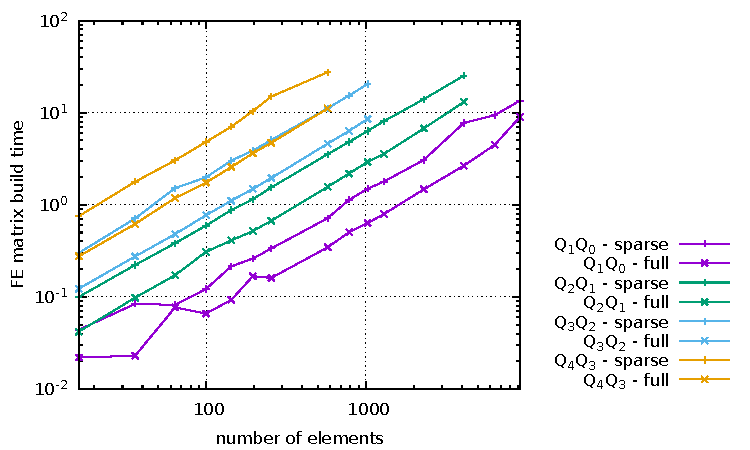
\includegraphics[height=6.cm]{python_codes/fieldstone_48/images/FEMbuildtimes.pdf}
\end{center}

Also not very surprising: the cost of building the FE matrix increases with the order
of the used elements. A matrix corresponding to 100 $Q_1\times P_0$ elements can be 
built in about 1s, while it will take 7s when $Q_4 \times Q_3$ elements are used. 



%-------------------------------------------------
\subsection*{Results with $Q_1\times P_0$ element}


\begin{center}
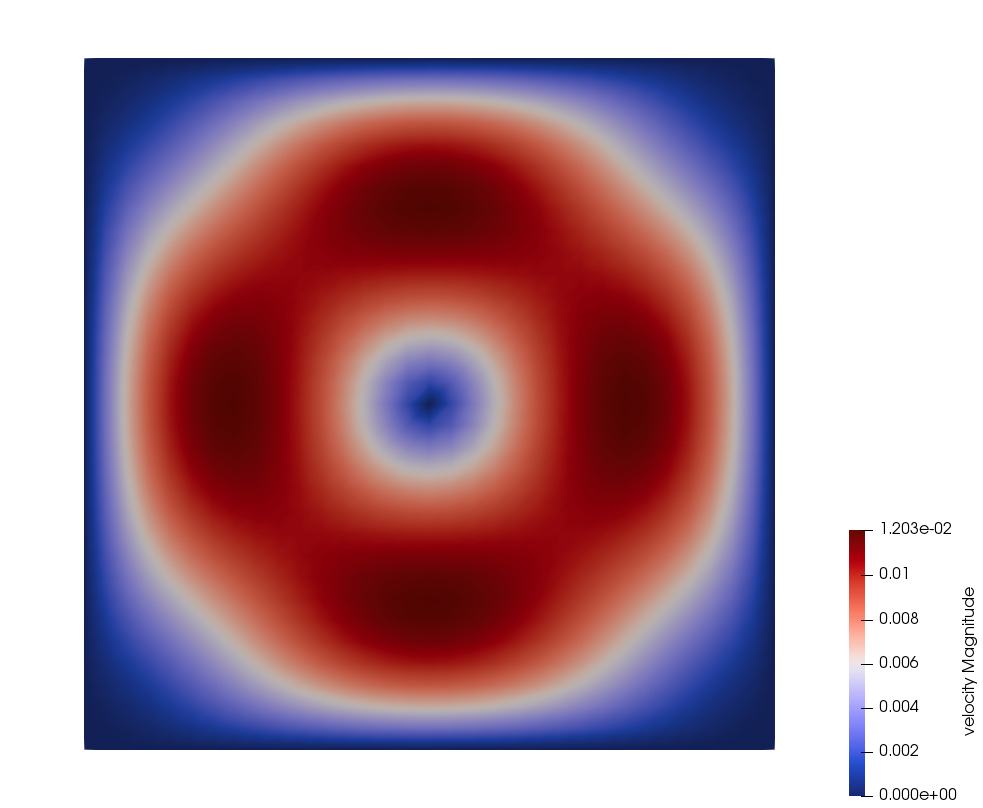
\includegraphics[height=6.cm]{python_codes/fieldstone_48/images/q1q0/vel}
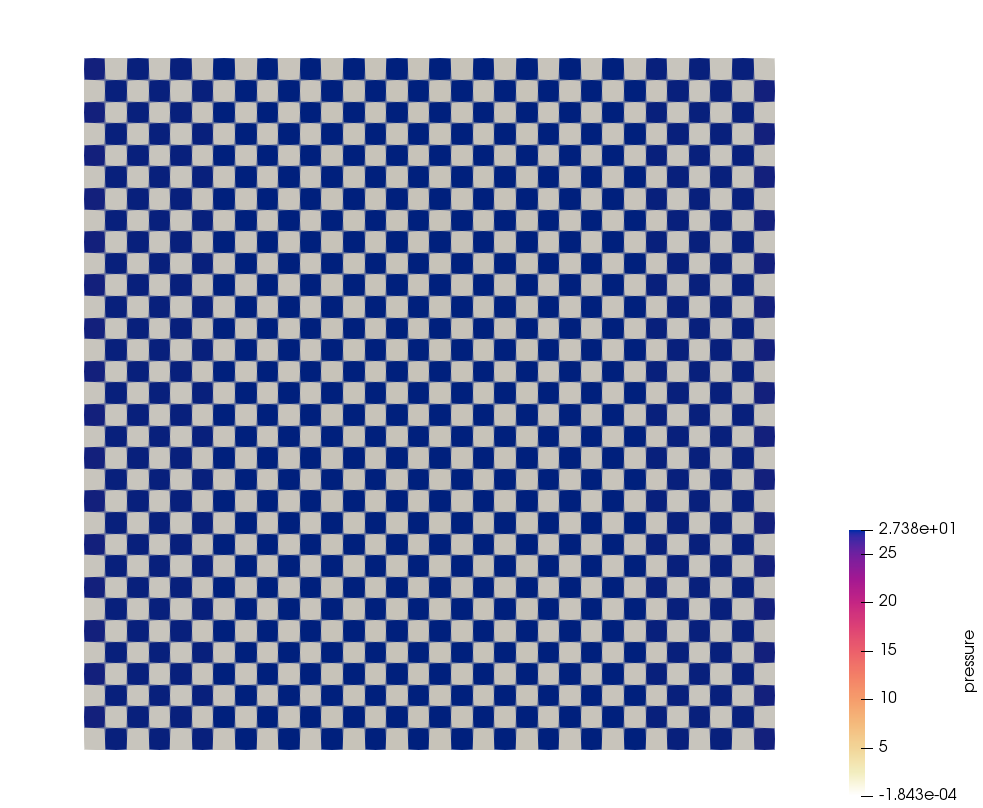
\includegraphics[height=6.cm]{python_codes/fieldstone_48/images/q1q0/p}\\
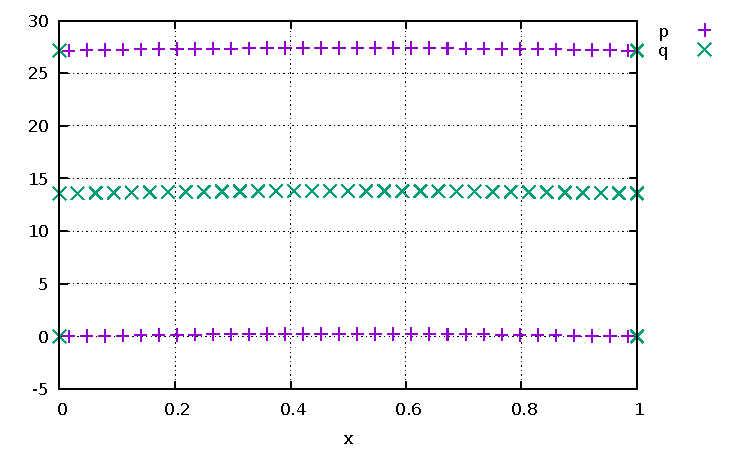
\includegraphics[height=4.cm]{python_codes/fieldstone_48/images/q1q0/pressure.pdf}
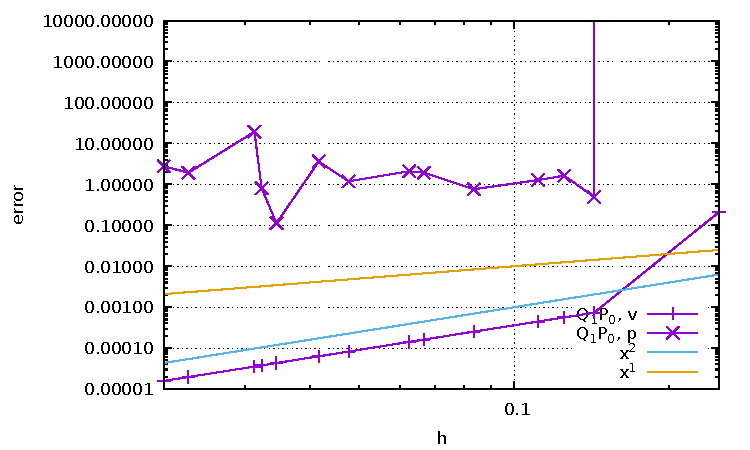
\includegraphics[height=4.cm]{python_codes/fieldstone_48/images/q1q0/errors1.pdf}
\end{center}

We see that we recover a second order convergence rate for velocity (as expected) 
but because of the checkerboard pattern the pressure convergence is simply random. 
The smoothed pressure $q$ shows virtually no checkerboard pattern, except on the boundaries.
This is a perfect example for the use of more accurate/clever smoothing procedure, see
Section~\ref{psmoothing}.


\subsection*{Results with $Q_2\times Q_1$ element}

We recover the cubic convergence for the velocity error and the quadratic convergence 
for the pressure:

\begin{center}
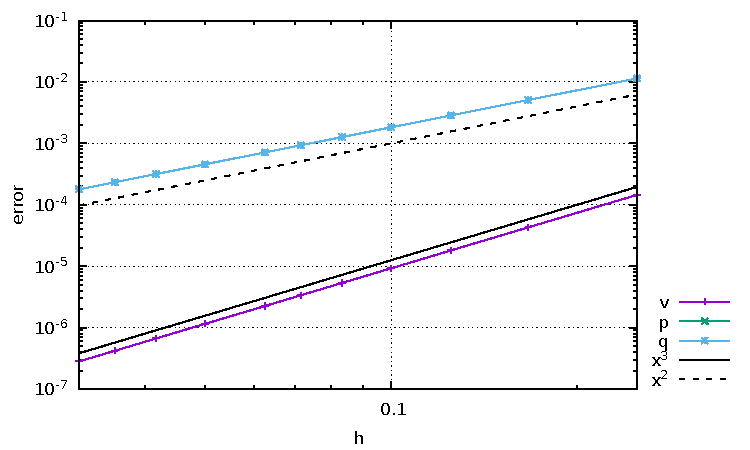
\includegraphics[width=8cm]{python_codes/fieldstone_48/images/errors2.pdf}
\end{center}

\subsection*{Results with $Q_3\times Q_2$ element}

The analytical solution is a second order polynomial, which means that the pressure 
shape functions can adequately represent the solution. We recover a fourth-order 
convergence for the velocity error and a superconvergent (fifth order) pressure error 
(but why is it 5th order ?).

\begin{center}
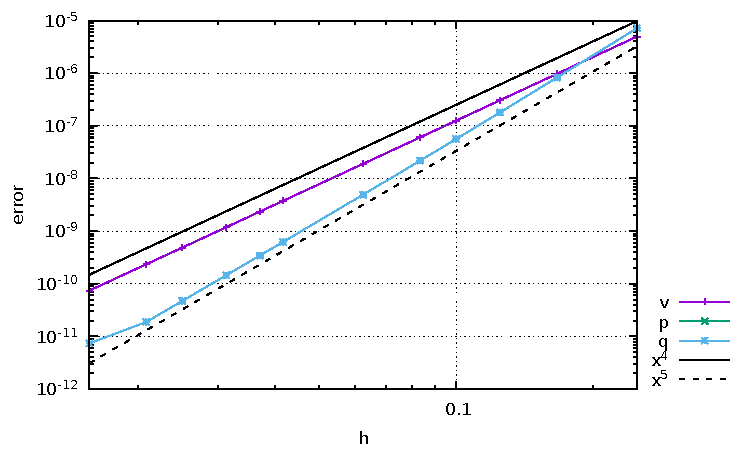
\includegraphics[width=8cm]{python_codes/fieldstone_48/images/errors3.pdf}
\end{center}

\subsection*{Results with $Q_4\times Q_3$ element}

Rather interestingly, now both velocity and pressure analytical solutions 
can be represented exactly by their respective polynomial spaces, so that 
the errors are at machine precision.

\begin{center}
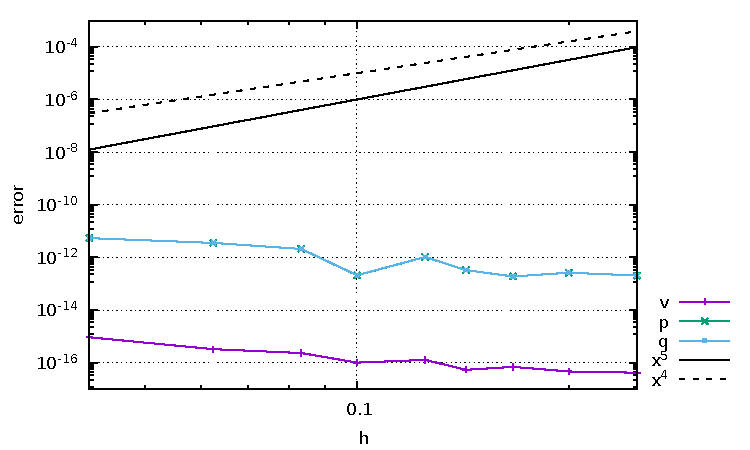
\includegraphics[width=8cm]{python_codes/fieldstone_48/images/errors4.pdf}
\end{center}



